\documentclass[tikz,border=6pt]{standalone}
\usepackage{amsmath}
\usepackage{xcolor}

% Màu ZO Math
\definecolor{zo_red}{HTML}{F44336}      % Red Salsa
\definecolor{zo_yellow}{HTML}{FFC107}   % Amber
\definecolor{zo_gray_bg}{HTML}{555555}
\definecolor{zo_white}{HTML}{FFFFFF}

\begin{document}

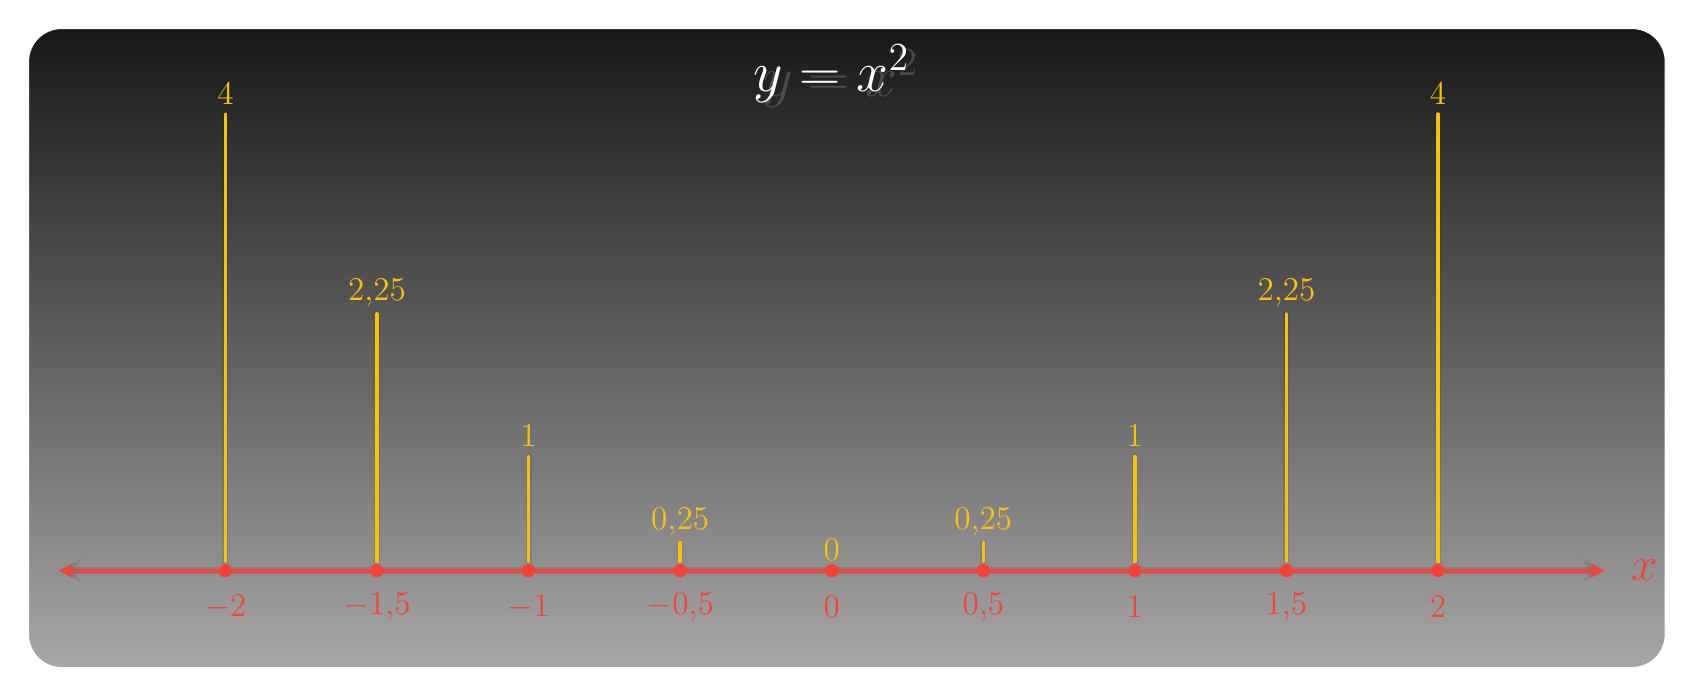
\begin{tikzpicture}[
  x=3.85cm,
  y=1.45cm,
  line cap=round,
  line join=round,
  >=stealth
]

% Kích thước khung ảnh
\def\xmin{-2.65}
\def\ymin{-0.85}
\def\xmax{2.75}
\def\ymax{4.75}

% Style
\tikzset{
  xaxis/.style={
    zo_red,
    line width=1.35pt,
    <->,
    preaction={draw, black, opacity=0.10, line width=2.5pt}
  },
  xdot/.style={
    fill=zo_red,
    draw=zo_red
  },
  stemy/.style={
    zo_yellow,
    line width=1.25pt,
    preaction={draw, black, opacity=0.08, line width=2.2pt}
  },
  xtext/.style={
    text=zo_red,
    font=\fontsize{13}{15}\selectfont
  },
  ytext/.style={
    text=zo_yellow,
    font=\fontsize{13}{15}\selectfont
  },
  coverformula/.style={
    text=zo_white,
    font=\fontsize{22}{26}\selectfont
  }
}

% =========================
% Khung nền bo góc + clip
% =========================
\begin{scope}
  \clip[rounded corners=12pt] (\xmin,\ymin) rectangle (\xmax,\ymax);

  % Nền gradient nhẹ
  \shade[
    top color=zo_gray_bg!28!black,
    bottom color=zo_gray_bg!52!white
  ] (\xmin,\ymin) rectangle (\xmax,\ymax);

  % =========================
  % Công thức (có bóng nhẹ)
  % =========================
  \node[coverformula, white, opacity=0.18] at (0.03,4.31) {$y=x^2$};
  \node[coverformula] at (0,4.35) {$y=x^2$};

  % =========================
  % Trục x
  % =========================
  \draw[xaxis] (-2.55,0) -- (2.55,0);
  \node[xtext, font=\fontsize{16}{18}\selectfont] at (2.68,0) {$x$};

  % =========================
  % Các giá trị x
  % =========================
  \foreach \x/\label in {
    -2/{-2},
    -1.5/{-1{,}5},
    -1/{-1},
    -0.5/{-0{,}5},
    0/{0},
    0.5/{0{,}5},
    1/{1},
    1.5/{1{,}5},
    2/{2}
  } {
    \node[xtext] at (\x,-0.32) {$\label$};
  }

  % =========================
  % Dấu chấm trên mỗi giá trị x
  % =========================
  \foreach \x in {-2,-1.5,-1,-0.5,0,0.5,1,1.5,2} {
    \fill[xdot] (\x,0) circle (2.2pt);
  }

  % =========================
  % Các đoạn thẳng đứng và giá trị y
  % =========================
  \def\ygap{0.08}

  \foreach \x/\y/\label in {
    -2/4/{4},
    -1.5/2.25/{2{,}25},
    -1/1/{1},
    -0.5/0.25/{0{,}25},
    0.5/0.25/{0{,}25},
    1/1/{1},
    1.5/2.25/{2{,}25},
    2/4/{4}
  } {
    \draw[stemy] (\x,\ygap) -- (\x,\y);
    \node[ytext] at (\x,\y+0.18) {$\label$};
  }

  % Giá trị y = 0 tại gốc
  \node[ytext, above] at (0,0) {$0$};

\end{scope}

% =========================
% Viền bo góc nhẹ
% =========================
\draw[
  rounded corners=12pt,
  line width=0.5pt,
  color=zo_white!42
] (\xmin,\ymin) rectangle (\xmax,\ymax);

\end{tikzpicture}

\end{document}